\begin{figure}[!h]
 \centering
 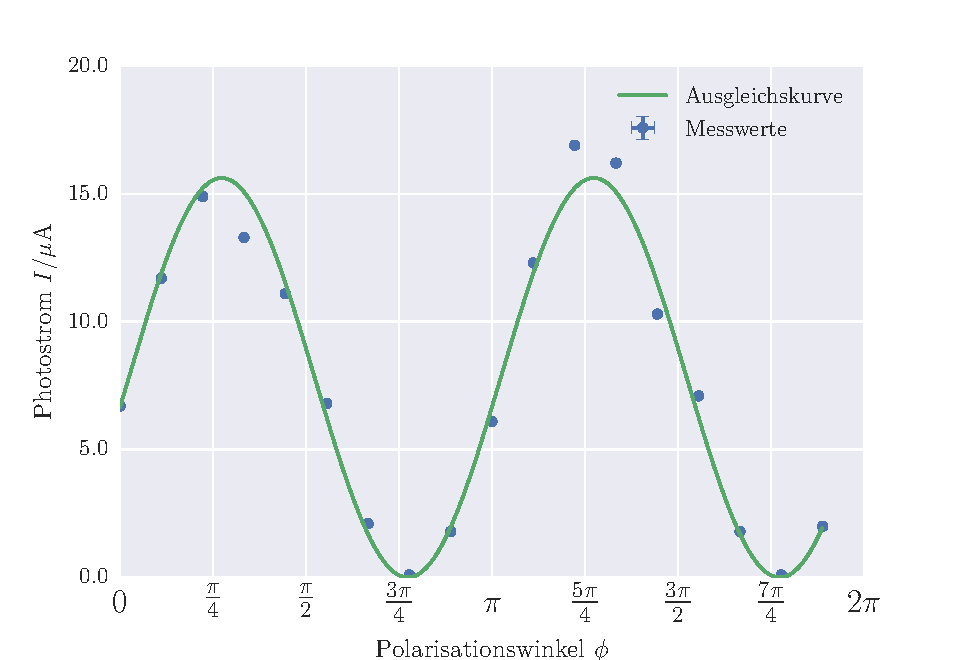
\includegraphics[scale=0.75]{../Grafiken/Polarisation.pdf}
 \caption{Grafische Darstellung der aufgenommenen Messwerte des Photostroms in Abhängigkeit des, am Polarisator eingestellten, Winkels. Die aufgenommenen Messfehler sind dabei in beiden 
 Dimensionen zu gering, um in der Grafik erkennbar zu sein.\label{fig:polarisation}}
 \end{figure} 